\documentclass[11pt]{article}

\usepackage{naaclhlt2012}
\usepackage{times}
\usepackage{latexsym}
\usepackage{amsmath}
\usepackage{multirow}
\usepackage{url}
\usepackage{graphicx}
\usepackage{subfig}
\usepackage{marvosym}

\setlength\titlebox{6.5cm}

\hyphenation{CachePipe}

%% \newcommand{\aff}{\ensuremath{{}^\text{\Radioactivity}}}
%% \newcommand{\afff}{\ensuremath{{}^\text{\Bat}}}
\newcommand{\aff}{\ensuremath{{}^\text{1}}}
\newcommand{\afff}{\ensuremath{{}^\text{2}}}
\newcommand{\grammarrule}[3]{$#1 \to \langle \text{#2} , \text{#3} \rangle$ }

\title{Joshua 3.0: Syntax-based Machine Translation \\ with the Thrax
  Grammar Extractor}

\author{Juri Ganitkevitch\aff, Yuan Cao\aff, Chris
  Callison-Burch\aff, Matt Post\afff, \and Jonathan Weese\aff \\
  \aff Center for Language and Speech Processing \\
  \afff Human Language Technology Center of Excellence \\
  Johns Hopkins University}

\date{}

\begin{document}
\maketitle

\begin{abstract}
  Pro, compact grammars, paraphrase pivoting 
  TODO Juri: write this
\end{abstract}

\section{Introduction}

TODO Juri: clean this up and flesh it out.

Joshua is an
open-source\footnote{\url{http://github.com/joshua-decoder/joshua}}
toolkit for hierarchical machine translation of human languages.  The
original version of Joshua \cite{Joshua-WMT} was a reimplementation of
the Python-based Hiero machine-translation system \cite{Chiang2007};
it was later extended \cite{li2010joshua} to support richer
formalisms, such as SAMT \cite{samt2006}.

\section{Compact Grammar Representation}

TODO Juri: intro into this part.

\subsection{Packed Synchronous Tries}

Memory usage is a limitation of both the Joshua and cdec
extractors. Translation models can be very large, and many feature
scores require accumulation of statistical data from the entire set of
extracted rules. Since it is impractical to keep the entire grammar in
memory, rules are usually sorted on disk and then read sequentially.

\subsubsection{Source-Side Trie}

TODO Juri: describe source-side format

\subsubsection{Target-Side Trie}

TODO Juri: describe target-side format

\subsubsection{Attached Data}

TODO Juri: discuss attached data idea, describe feature format,
alignments

\subsection{Quantization}

TODO Juri: discuss features taking the most spaces, quantization in
the spirit of KenLM and BerkeleyLM.

\subsection{Optimizations}

TODO Juri: what did we do to improve decoding speed?

\subsection{Experiments}

TODO Juri: brief rundown of experiments

\begin{figure}[!t]
\begin{center}

\includegraphics[width=0.4\linewidth]{figures/placeholder.jpeg}
\end{center}
\caption{TODO Juri: Decoding versus load time plot.}
\label{fig-example-compression}
\end{figure}

\begin{table}
\centering
\begin{tabular}{|c|c|c|}
Language pair & sentences (K) & words (M) \\
\hline\hline
cs--en & 332 & 4.7 \\
de--en & 279 & 5.5 \\
en--cs & 487 & 6.9 \\
en--de & 359 & 7.2 \\
en--fr & 682 & 12.5 \\
fr--en & 792 & 14.4 \\
\end{tabular}
\caption{TODO Juri: some BLEU scores for quantized versus not quantized.}
\end{table}


<<<<<<< HEAD
\section{J-PRO: Pairwise Ranking Optimization in Joshua}
\label{section:results}
\subsection{PRO Overview} \label{section:pro-overview}
Pairwise ranking optimization(PRO) proposed by \cite{Hopkins2011} is a new method for statistical machine translation discriminative parameter tuning. It is reported to be more stable than the popular MERT algorithm\cite{Och2003} and is more scalable with the feature dimensionality. PRO treats the parameter tuning problem as $n$-best list reranking problem, and the idea is similar to other pairwise ranking techniques like ranking SVM and IR SVM \cite{Hang2011}. We briefly describe the algorithm as the following.

Let $h(c)=\langle \mathbf{w},\mathbf{\Phi}(c)\rangle$ be the linear model score of a candidate translation $c$, in which $\mathbf{\Phi}(c)$ is the feature vector of $c$ and $\mathbf{w}$ is the parameter vector. Also let $g(c)$ be the metric score of $c$(without loss of generality, assuming higher score indicates better translation). We hope to find a parameter vector $\mathbf{w}$ such that for a pair of candidates $\{ c_i,c_j \}$ in an $n$-best list, $(h(c_i)-h(c_j))(g(c_i)-g(c_j))=\langle \mathbf{w},\mathbf{\Phi}(c_i) - \mathbf{\Phi}(c_j)\rangle (g(c_i)-g(c_j)) >0$, namely the order of the model score is consistent with that of the metric score. This can be turned into a binary classification problem, by adding instance $\Delta\mathbf{\Phi}_{ij}=\mathbf{\Phi}(c_i) - \mathbf{\Phi}(c_j)$ with class label $sign(g(c_i)-g(c_j))$ to the training data(and symmetrically add instance $\Delta\mathbf{\Phi}_{ji}=\mathbf{\Phi}(c_j) - \mathbf{\Phi}(c_i)$ with class label $sign(g(c_j)-g(c_i))$ at the same time), then using any binary classifier to find the $\mathbf{w}$ which determines a hyperplane separating the two classes(therefore the performance of PRO depends on the choice of classifier to a large extent). Given a training set with $T$ sentences, there are $O(Tn^2)$ pairs of candidates that can be added to the training set, this number is usually too huge for efficient training. To make the task more tractable, PRO samples a subset of the candidate pairs so that only those pairs whose metric score difference is large enough are qualified as training instances. This follows the intuition that high score differential makes it easier to separate good translations from bad ones.

\subsection{Description of J-PRO} \label{section:j-pro}
PRO is implemented in Joshua 4.0 named J-PRO. In order to ensure compatibility with the decoder and the parameter tuning module Z-MERT \cite{zaidan2009z} included in all versions of Joshua, J-PRO is built upon the architecture of Z-MERT with similar usage and configuration files(with a few extra lines specifying PRO-related parameters), and inherited from Z-MERT the favorable feature of easy metric plug-in. Since PRO allows using any off-the-shelf binary binary classifiers, J-PRO provides a Java interface that enables easy plug-in of any classifier. The current version of J-PRO supports three classifiers by implementing this interface:

 \emph{Perceptron} \cite{Rosenblatt1958}: the perceptron is self-contained in J-PRO, no external resources required.

 \emph{MegaM} \cite{Hal2004}: the classifier used in \cite{Hopkins2011}.

 \emph{Maximum entropy classifier}: the Stanford toolkit of maximum entropy classifier.\footnote{Available at \url{http://nlp.stanford.edu/software/classifier.shtml}}
  
The user may specify which classifier he wants to use and the classifier-specific parameters in the J-PRO configuration file.

To take the advantage of PRO's ability of handling large number of features, J-PRO supports training with dense and sparse features. When both dense and sparse features are involved in training, sometimes it is not a good practice to directly tune parameters for these two kinds of heterogeneous features, as dense features may bring side effects to the training process when combined with sparse features \cite{Kristy2008}. To better handle the relation between dense and sparse features and provide more flexible training schemes, J-PRO supports four training modes(suppose $M$ dense features and $N$ sparse features are used):

\emph{Mode 1}: tune the dense feature parameters only, just like Z-MERT($M$ parameters to tune).

\emph{Mode 2}: tune the dense + sparse feature parameters together($M+N$ parameters to tune).

\emph{Mode 3}: tune the sparse feature parameters only with the dense feature parameters fixed, and sparse feature parameters scaled by a manually specified constant($N$ parameters to tune).

\emph{Mode 4}: tune the dense feature parameters and the scaling factor for sparse features, with the sparse feature parameters fixed($M$+1 parameters to tune).

J-PRO supports $n$-best list input with sparse feature format which enumerates only the firing features together with their values, to enable compact feature representation when numerous features are involved in training.

\subsection{Experiments}
We did our experiments using J-PRO on the NIST Chinese-English data, and BLEU score was used as the quality metric for experiments reported in this section.\footnote{We also exprimented with other metrics including TER, METEOR and TER-BLEU. Similar trends as reported in this section were observed. These results are omitted here due to limited space.} The experimental settings are as the following:

\emph{Datasets}: MT03 dataset(998 sentences) as development set for parameter tuning, MT04(1788 sentences) and MT05(1082 sentences) as test sets. 

\emph{Features}: Dense feature set include the 10 regular features used in the Hiero system; Sparse feature set includes 1016 target-side rule POS bi-gram features as used in \cite{Li2010coling}.

\emph{Classifiers}: Perceptron, Megam and Maximum entropy.

\emph{PRO parameters}: $\Gamma=8000$(number of candidate pairs sampled uniformly from the $n$-best list), $\alpha=1$(sample acceptance probability), $\Xi=50$(number of top candidates to be added to the training set).

Fig.\ref{fig:pro1} shows the BLEU score curves on the development and test sets as a function of iterations. The upper and lower rows correspond to the results trained with 10 dense features and 1026 dense+sparse features respectively. We intentionally selected very bad initial parameter vectors to verify the robustness of the algorithm. It can be seen that as the iteration goes on, the BLEU scores increase monotonically on both development and test sets, and start to converge after a few iterations. When only 10 features are involved, all classifiers give almost the same performance. However, when scaled to over a thousand features, the maximum entropy classifier becomes unstable and the curve fluctuates significantly. In this situation MegaM behaves well, but the J-PRO built-in perceptron gives the most robust performance. 

Table\ref{table:pro} makes a comparison between the results given by Z-MERT and J-PRO. Since MERT is not able to handle numerous sparse features, only results trained with 10 features are shown. The scores given by both results are quite close to each other, Z-MERT did slightly better on the development set but J-PRO did slightly better on the test set.

\begin{figure*}[htbp]
\begin{center}$
\begin{array}{ccc}
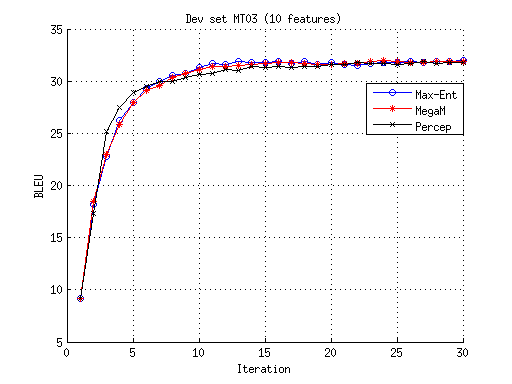
\includegraphics[width=0.3\textwidth]{figures/mt03_10feat.png}
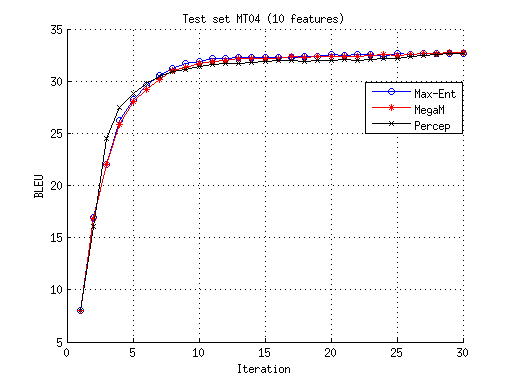
\includegraphics[width=0.3\textwidth]{figures/mt04_10feat.png}
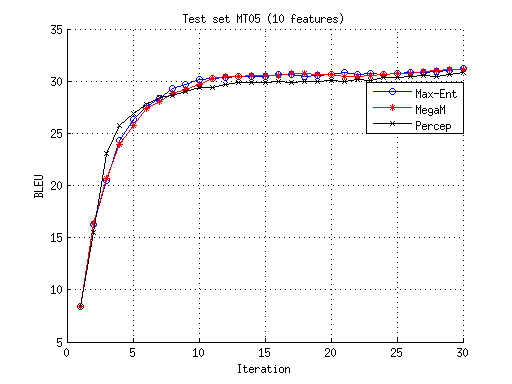
\includegraphics[width=0.3\textwidth]{figures/mt05_10feat.png}\\
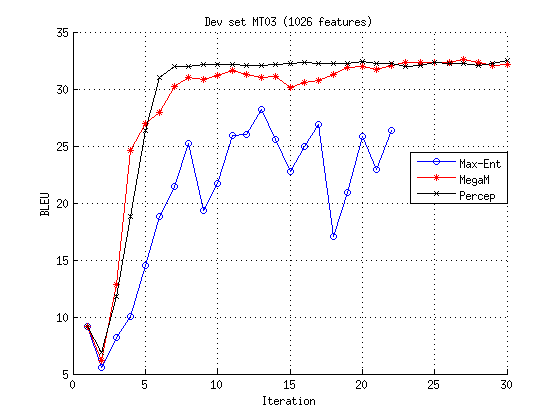
\includegraphics[width=0.3\textwidth]{figures/mt03_1026feat.png}
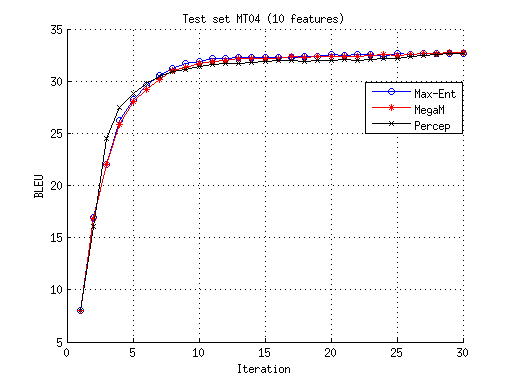
\includegraphics[width=0.3\textwidth]{figures/mt04_10feat.png}
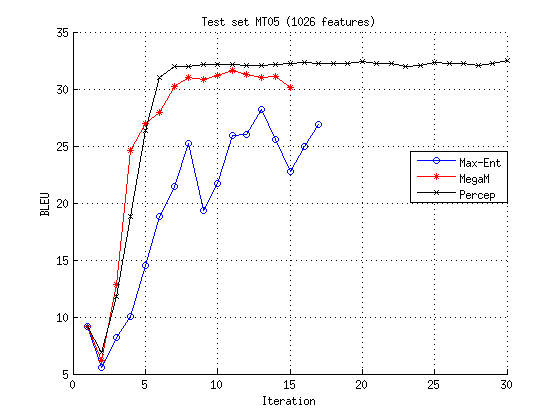
\includegraphics[width=0.3\textwidth]{figures/mt05_1026feat.png}
\end{array}$
\end{center}
\caption{\label{fig:pro1}Experimental results on the development and test sets. The $x$-axis is the number of iterations(up to 30) and the $y$-axis is the BLEU score. The three curves in each figure correspond to three classifiers. Upper row: results trained using only dense features(10 features); Lower row: results trained using dense+sparse features(1026 features). Left column: development set(MT03); Middle column: test set(MT04); Right column: test set(MT05).}
\end{figure*}

\begin{table}
\centering
\begin{tabular}{|c|c|c|c|c|}
\multirow{2}{*}{Datasets} & \multirow{2}{*}{Z-MERT} & \multicolumn{3}{c}{PRO} \\
            &       &Percep &MegaM &Max-Ent\\
\hline\hline
Dev(MT03)   &32.23  &31.85  &32     &31.98\\
Test(MT04)  &32.56  &32.65  &32.65  &32.55\\
Test(MT05)  &30.68  &30.87  &31     &30.89\\
\end{tabular}
\caption{\label{table:pro} Comparison between the results given by Z-MERT and J-PRO(trained with 10 features).}
=======
\section{Y-PRO: Pairwise Ranking Optimization in Joshua}
\label{section:results}

TODO Yuan: give a brief description of PRO, highlight the
compatibility with Z-MERT's easily plugged in metrics. Also highlight
the supported classifiers (which we should fix in the main repository) 

\subsection{Experiments}

TODO Yuan: Describe the experiments you did for
convergence/speed/translation quality

\begin{figure}[!t]
\begin{center}

\includegraphics[width=0.4\linewidth]{figures/placeholder.jpeg}
\end{center}
\caption{TODO Yuan: Plot of iterations/score for various classifiers,
  pointing out that our built-in perceptron is doing well.}
\label{fig-example-compression}
\end{figure}

\begin{table}
\centering
\begin{tabular}{|c|c|c|}
Language pair & sentences (K) & words (M) \\
\hline\hline
cs--en & 332 & 4.7 \\
de--en & 279 & 5.5 \\
en--cs & 487 & 6.9 \\
en--de & 359 & 7.2 \\
en--fr & 682 & 12.5 \\
fr--en & 792 & 14.4 \\
\end{tabular}
\caption{TODO Yuan: Table of MERT versus PRO (with various
  classifiers) showing numer of iterations, time needed and scores on
  dev and test.}
>>>>>>> 16400e4dea2b9355b8c7e2fdfa80cd4d6e843fe2
\end{table}


\section{Thrax: Paraphrase Extraction at Scale}

TODO Juri: describe paraphrase stage and integration with Thrax
features

\begin{table}
\centering
\begin{tabular}{|c|c|c|}
Language pair & sentences (K) & words (M) \\
\hline\hline
cs--en & 332 & 4.7 \\
de--en & 279 & 5.5 \\
en--cs & 487 & 6.9 \\
en--de & 359 & 7.2 \\
en--fr & 682 & 12.5 \\
fr--en & 792 & 14.4 \\
\end{tabular}
\caption{TODO Juri: Table of large grammars we extracted.}
\end{table}

\section{Future work}

<<<<<<< HEAD
%TODO All: Ideas? Sparse features?
(Possibly more flexible/convenient definition of sparse features in the decoder.)
=======
TODO All: Ideas? Sparse features?
>>>>>>> 16400e4dea2b9355b8c7e2fdfa80cd4d6e843fe2


% \section*{Acknowledgements}
% This research was supported by in part by the EuroMatrixPlus project
% funded by the European Commission (7th Framework Programme), and by
% the NSF under grant IIS-0713448. Opinions, interpretations, and
% conclusions are the authors' alone.

\bibliographystyle{naaclhlt2012}
\bibliography{joshua}

\end{document}
